\documentclass[11pt]{article}

\newcommand{\yourname}{Kevin Zhang}

\def\comments{0}

%format and packages

%\usepackage{algorithm, algorithmic}
\usepackage{forest}
\usepackage{tikz}
\usepackage{algpseudocode}
\usepackage{amsmath, amssymb, amsthm}
\usepackage{tcolorbox}
\usepackage{enumerate}
\usepackage{enumitem}
\usepackage{framed}
\usepackage{verbatim}
\usepackage[margin=1.0in]{geometry}
\usepackage{microtype}
\usepackage{kpfonts}
\usepackage{palatino}
	\DeclareMathAlphabet{\mathtt}{OT1}{cmtt}{m}{n}
	\SetMathAlphabet{\mathtt}{bold}{OT1}{cmtt}{bx}{n}
	\DeclareMathAlphabet{\mathsf}{OT1}{cmss}{m}{n}
	\SetMathAlphabet{\mathsf}{bold}{OT1}{cmss}{bx}{n}
	\renewcommand*\ttdefault{cmtt}
	\renewcommand*\sfdefault{cmss}
	\renewcommand{\baselinestretch}{1.06}

\usepackage[boxruled,vlined,nofillcomment]{algorithm2e}
	\SetKwProg{Fn}{Function}{\string:}{}
	\SetKwFor{While}{While}{}{}
	\SetKwFor{For}{For}{}{}
	\SetKwIF{If}{ElseIf}{Else}{If}{:}{ElseIf}{Else}{:}
	\SetKw{Return}{Return}
\usepackage{listings}% http://ctan.org/pkg/listings
\lstset{
  basicstyle=\ttfamily,
  mathescape
}		
\usetikzlibrary{shapes.geometric, arrows}
\usetikzlibrary{positioning}

%enclosure macros
\newcommand{\paren}[1]{\ensuremath{\left( {#1} \right)}}
\newcommand{\bracket}[1]{\ensuremath{\left\{ {#1} \right\}}}
\renewcommand{\sb}[1]{\ensuremath{\left[ {#1} \right\]}}
\newcommand{\ab}[1]{\ensuremath{\left\langle {#1} \right\rangle}}

%probability macros
\newcommand{\ex}[2]{{\ifx&#1& \mathbb{E} \else \underset{#1}{\mathbb{E}} \fi \left[#2\right]}}
\newcommand{\pr}[2]{{\ifx&#1& \mathbb{P} \else \underset{#1}{\mathbb{P}} \fi \left[#2\right]}}
\newcommand{\var}[2]{{\ifx&#1& \mathrm{Var} \else \underset{#1}{\mathrm{Var}} \fi \left[#2\right]}}

%useful CS macros
\newcommand{\poly}{\mathrm{poly}}
\newcommand{\polylog}{\mathrm{polylog}}
\newcommand{\zo}{\{0,1\}}
\newcommand{\pmo}{\{\pm1\}}
\newcommand{\getsr}{\gets_{\mbox{\tiny R}}}
\newcommand{\card}[1]{\left| #1 \right|}
\newcommand{\set}[1]{\left\{#1\right\}}
\newcommand{\negl}{\mathrm{negl}}
\newcommand{\eps}{\varepsilon}
\DeclareMathOperator*{\argmin}{arg\,min}
\DeclareMathOperator*{\argmax}{arg\,max}
\newcommand{\eqand}{\qquad \textrm{and} \qquad}
\newcommand{\ind}[1]{\mathbb{I}\{#1\}}
\newcommand{\sslash}{\ensuremath{\mathbin{/\mkern-3mu/}}}
\newcommand{\pipe}{\hspace{3pt}|\hspace{3pt}}

%mathbb
\newcommand{\N}{\mathbb{N}}
\newcommand{\R}{\mathbb{R}}
\newcommand{\Z}{\mathbb{Z}}
%mathcal
\newcommand{\cA}{\mathcal{A}}
\newcommand{\cB}{\mathcal{B}}
\newcommand{\cC}{\mathcal{C}}
\newcommand{\cD}{\mathcal{D}}
\newcommand{\cE}{\mathcal{E}}
\newcommand{\cF}{\mathcal{F}}
\newcommand{\cL}{\mathcal{L}}
\newcommand{\cM}{\mathcal{M}}
\newcommand{\cO}{\mathcal{O}}
\newcommand{\cP}{\mathcal{P}}
\newcommand{\cQ}{\mathcal{Q}}
\newcommand{\cR}{\mathcal{R}}
\newcommand{\cS}{\mathcal{S}}
\newcommand{\cU}{\mathcal{U}}
\newcommand{\cV}{\mathcal{V}}
\newcommand{\cW}{\mathcal{W}}
\newcommand{\cX}{\mathcal{X}}
\newcommand{\cY}{\mathcal{Y}}
\newcommand{\cZ}{\mathcal{Z}}

%theorem macros
\newtheorem{thm}{Theorem}
\newtheorem{lem}[thm]{Lemma}
\newtheorem{fact}[thm]{Fact}
\newtheorem{clm}[thm]{Claim}
\newtheorem{rem}[thm]{Remark}
\newtheorem{coro}[thm]{Corollary}
\newtheorem{prop}[thm]{Proposition}
\newtheorem{conj}[thm]{Conjecture}

\theoremstyle{definition}
\newtheorem{defn}[thm]{Definition}
\newtheoremstyle{case}{}{}{}{}{}{:}{ }{}
\theoremstyle{case}
\newtheorem{case}{Case}

\theoremstyle{theorem}
\newtheorem{prob}{Problem}
\newtheorem{sol}{Solution}

\tikzset{every picture/.style={line width=0.75pt}} %set default line width to 0.75pt        

\begin{document}
{\large
\noindent Name: \yourname}

\vspace{15pt}

\begin{prob}\end{prob}



\tikzset{every picture/.style={line width=0.75pt}} %set default line width to 0.75pt        

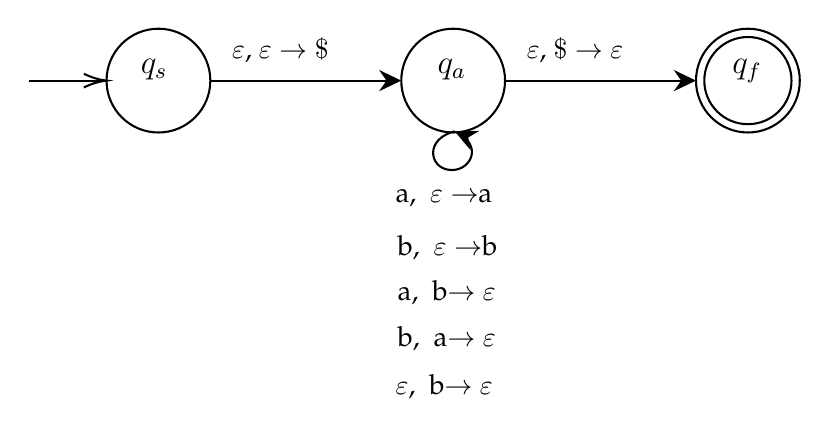
\begin{tikzpicture}[x=0.75pt,y=0.75pt,yscale=-1,xscale=1]
%uncomment if require: \path (0,216); %set diagram left start at 0, and has height of 216

%Shape: Circle [id:dp453385868393156] 
\draw   (58,41) .. controls (58,27.19) and (69.19,16) .. (83,16) .. controls (96.81,16) and (108,27.19) .. (108,41) .. controls (108,54.81) and (96.81,66) .. (83,66) .. controls (69.19,66) and (58,54.81) .. (58,41) -- cycle ;
%Shape: Circle [id:dp39205866177721194] 
\draw   (200,41) .. controls (200,27.19) and (211.19,16) .. (225,16) .. controls (238.81,16) and (250,27.19) .. (250,41) .. controls (250,54.81) and (238.81,66) .. (225,66) .. controls (211.19,66) and (200,54.81) .. (200,41) -- cycle ;
%Straight Lines [id:da6227939795417778] 
\draw    (20.5,41) -- (56,41) ;
\draw [shift={(58,41)}, rotate = 180] [color={rgb, 255:red, 0; green, 0; blue, 0 }  ][line width=0.75]    (10.93,-3.29) .. controls (6.95,-1.4) and (3.31,-0.3) .. (0,0) .. controls (3.31,0.3) and (6.95,1.4) .. (10.93,3.29)   ;
%Straight Lines [id:da019534467811933354] 
\draw    (108,41) -- (197,41) ;
\draw [shift={(200,41)}, rotate = 180] [fill={rgb, 255:red, 0; green, 0; blue, 0 }  ][line width=0.08]  [draw opacity=0] (10.72,-5.15) -- (0,0) -- (10.72,5.15) -- (7.12,0) -- cycle    ;
%Curve Lines [id:da8695220076332031] 
\draw    (225.78,65.44) .. controls (211.28,69.04) and (213.28,83.04) .. (223.28,84.04) .. controls (232.63,84.98) and (239.35,73.67) .. (228.34,66.8) ;
\draw [shift={(225.78,65.44)}, rotate = 384.47] [fill={rgb, 255:red, 0; green, 0; blue, 0 }  ][line width=0.08]  [draw opacity=0] (10.72,-5.15) -- (0,0) -- (10.72,5.15) -- (7.12,0) -- cycle    ;
%Shape: Circle [id:dp24865571582265633] 
\draw   (342,41) .. controls (342,27.19) and (353.19,16) .. (367,16) .. controls (380.81,16) and (392,27.19) .. (392,41) .. controls (392,54.81) and (380.81,66) .. (367,66) .. controls (353.19,66) and (342,54.81) .. (342,41) -- cycle ;
%Straight Lines [id:da8869608812882375] 
\draw    (250,41) -- (339,41) ;
\draw [shift={(342,41)}, rotate = 180] [fill={rgb, 255:red, 0; green, 0; blue, 0 }  ][line width=0.08]  [draw opacity=0] (10.72,-5.15) -- (0,0) -- (10.72,5.15) -- (7.12,0) -- cycle    ;
%Shape: Circle [id:dp927082876757759] 
\draw   (346,41) .. controls (346,29.4) and (355.4,20) .. (367,20) .. controls (378.6,20) and (388,29.4) .. (388,41) .. controls (388,52.6) and (378.6,62) .. (367,62) .. controls (355.4,62) and (346,52.6) .. (346,41) -- cycle ;

% Text Node
\draw (73,29) node [anchor=north west][inner sep=0.75pt]  [font=\large] [align=left] {$\displaystyle q_{s}$};
% Text Node
\draw (216,29) node [anchor=north west][inner sep=0.75pt]  [font=\large] [align=left] {$\displaystyle q_{a}$};
% Text Node
\draw (117,19) node [anchor=north west][inner sep=0.75pt]   [align=left] {$\displaystyle \varepsilon $, $\displaystyle \varepsilon \rightarrow \$$};
% Text Node
\draw (195.77,91.97) node [anchor=north west][inner sep=0.75pt]   [align=left] {a, \ $\displaystyle \varepsilon \rightarrow $a};
% Text Node
\draw (358,29) node [anchor=north west][inner sep=0.75pt]  [font=\large] [align=left] {$\displaystyle q_{f}$};
% Text Node
\draw (259,19) node [anchor=north west][inner sep=0.75pt]   [align=left] {$\displaystyle \varepsilon $, $\displaystyle \$\rightarrow \varepsilon $};
% Text Node
\draw (196.77,113.97) node [anchor=north west][inner sep=0.75pt]   [align=left] {b, \ $\displaystyle \varepsilon \rightarrow $b};
% Text Node
\draw (196.77,135.97) node [anchor=north west][inner sep=0.75pt]   [align=left] {a, \ b$\displaystyle \rightarrow \varepsilon $};
% Text Node
\draw (196.77,157.97) node [anchor=north west][inner sep=0.75pt]   [align=left] {b, \ a$\displaystyle \rightarrow \varepsilon $};
% Text Node
\draw (195.77,180.97) node [anchor=north west][inner sep=0.75pt]   [align=left] {$\displaystyle \varepsilon $, \ b$\displaystyle \rightarrow \varepsilon $};


\end{tikzpicture}


The components are $q_s$, $q_a$, and $q_f$. $q_s$ is the start state, and simply puts a dollar
on the stack, which will get used later to determine when we reached the bottom of the stack.
$q_a$ does two things: match $a$ with $b$ as they show up, and discard any extra $b$s at the
end. Once we've reached the bottom of the stack (indicated by the dollar), we can safely 
transition to $q_f$ and accept. $q_a$'s first four transitions are to deal with scenarios
in which the $a$ shows up before the $b$ (or vice versa), or multiple $a$s shows up before the 
next $b$ (or vice versa). After everything is read, if every $b$ is used to wipe out a $a$ 
(and vice versa), the stack should end up with only $b$s, or empty (with dollar). The last 
transition of $q_a$ is to discard excess $b$s.

\begin{prob}\end{prob}

Left empty -- submitted online

\begin{prob}\end{prob}

\begin{enumerate}[label=(\alph*)]

\item 

The transitions of $M$ are:

\begin{lstlisting}
($s$ 0) ($s$ 1 S) 
($s$ 1) ($q_{accept}$ 0 L)
($s$ $\text{\textvisiblespace}$) ($q_{reject}$ 1 S)
\end{lstlisting}

\item

$M$ accepts all non-empty strings. If the string starts with 1, it replaces the 1 with a 0.
Otherwise, it converts 0 to 1, and then back to 0. In both cases, $M$ end in $q_{accept}$ 
with the head to the left of the first cell. $M$ rejects when the string is empty (and writes 
a 1, but that's not as important as rejecting.)

\item

$M$ is a decider. $M$ never looks beyond the first character. If the first character is
$\text{\textvisiblespace}$, then it rejects. If the first character is 0, then it 
flip-flops to 1, back to 0, and then it accepts. If the first character is 1, then it
converts it to 0, and accepts. In all cases, $M$ halts.

\end{enumerate}

\newpage

\begin{prob}\end{prob}

\begin{enumerate}[label=\arabic*.]

\item $A$ and $B$ are DFAs, which makes $L(A)$ and $L(B)$ regular languages

\item $L(A)$ and $L(B)$ have pumping lengths $p_A$ and $p_B$ that satisfy the pumping lemma
(they are both regular languages).

\item Pick $p$ to whichever $p_A$ or $p_B$ is greater. The Pumping Lemma states that
in a regular language $L$, there is a pumping length $p$ such that $w \in L$, where $|w| \geq p$ 
and $w = xyz$, where $y \neq \varepsilon$. Then $w_{pumped} = xy^nz$ where $n \in \N$ and 
$w_{pumped} \in L$. 

\item This means that after length $p$, all words in a language $L$ can be pumped from some word of length $p$.
This applies to both $L(A)$ and $L(B)$.

\item We picked $p$ to be the greater of $p_A$ and $p_B$. So after length $p$, 
all words in $L(A) \subseteq L(B)$. This means that the words $|w| \leq p$ are
the only ones we have to test.

\item DFAs accept only if a word is in a regular language, so, we can test the DFAs 
for strings of length $k \leq p$.

\end{enumerate}

\begin{prob}\end{prob}

\begin{enumerate}[label=(\alph*)]

\item Let 
ODD-SELF = \{ $\langle$ M $\rangle$ | M is a Turing machine that halts on input $\langle$ M $\rangle$ after an odd number of steps \}

Assume ODD-SELF is decidable by Turing Machine $T$. 

We can use diagonalization to construct a $D$ like so. 

\begin{tabular}{|c||c|c|c|}

$M_i$ halts on $\langle$ $M_i$ $\rangle$ after odd steps & $M_0$ & $M_1$ & $\hdots$ \\

\hline
\hline

$\langle$ $M_0$ $\rangle$ & yes & $\hdots$ & $\hdots$ \\

\hline

$\langle$ $M_1$ $\rangle$ & $\hdots$ & no & $\hdots$ \\

\hline

$\vdots$ & $\hdots$ & $\hdots$ & $\ddots$ \\

\hline
\hline

$D$ & no & yes & $\hdots$ \\

\end{tabular}

This will create a $D \neq M_1, M_2, M_3, ...$. We can program $D$ by doing the following:

\begin{enumerate}[label=(\alph*)]

\item On input $w \in \Sigma^*$, if $w$ is not encoding, do anything

\item If $w$ is encoding, then run $T$ on $w$, and add one more step (such as a stay-put). 
This will accept if $T$ reject, reject if $T$ accept. 

\end{enumerate}

This creates a contradiction, because if we run $D$ on $\langle D \rangle$, we 
end up with a situation such that both $D$ accepts and rejects, which means that $T$ is 
contradictory.

\newpage

\item

Yes. We can build a recognizer as follows:

\tikzstyle{process} = [rectangle, minimum width=3cm, minimum height=1cm, text centered, draw=black]
\tikzstyle{decision} = [diamond, minimum width=3cm, minimum height=1cm, text centered, draw=black]
\tikzstyle{arrow} = [thick,->,>=stealth]

\begin{tikzpicture}[node distance=2cm]

\node (input) [process] {Input w};

\node (dec1) [decision, below=of input, yshift=-0.5cm] {w = $\langle M \rangle$ for some $M$?};

\node (reject) [process, right=of dec1, xshift=2cm] {reject};

\node (accept) [process, below=of dec1, yshift=-0.5cm] {Run $M$ on $\langle M \rangle$};

\node (faccept) [process, below=of accept] {accept w};

\draw [arrow] (input) -- (dec1);

\draw [arrow] (dec1) -- node [anchor=south] {no} (reject);

\draw [arrow] (dec1) -- node [anchor=east] {yes} (accept);

\draw [arrow] (accept) -- node [anchor=east] {$M$ halts on $\langle M \rangle$ after odd steps?} (faccept);

\end{tikzpicture}

\item

The language ODD-HALT is not decidable. Assume (for contradiction), that ODD-HALT is decidable. 
Then, we can write a machine that takes $\langle M, \langle M \rangle \rangle$, where $w$ is now $\langle M \rangle$.
This means that if ODD-HALT is decidable, then ODD-SELF must be decidable. But, we've proven
that ODD-SELF is not deciable. Thus, ODD-HALT is not decidable.

\end{enumerate}

\newpage

\begin{prob}\end{prob}

\begin{enumerate}[label=(\alph*)]

\item Undecidable. There are some languages such that $1011 \in L(M_1)$. 
There are some languages such that $1011 \notin L(M_2)$. As such, the property is non-trivial,
and is a property of the languages of $M_1$ and $M_2$. Therefore, we can use Rice's theorem
to show that this is undecidable.

\item Undecidable. There are some langauges that accept all input, so $L(M_1) = \Sigma^*$. 
There are also some languages that will reject some input, so $L(M_2) \neq \Sigma^*$. As such,
the property is non-trivial, and the property is a property of the languages. Therefore,
we can use Rice's theorem to show that this is undecidable.

\item Undecidable. There are some langauges that reject all input, so $L(M_1) = \varnothing$. 
There are also some languages that will accept some input, so $L(M_2) \neq \varnothing$. As such,
the property is non-trivial, and the property is a property of the languages. Therefore,
we can use Rice's theorem to show that this is undecidable.

\end{enumerate}

\begin{prob}\end{prob}

Yes. To put it another way, Self-$A_{TM}$ can be written as 

\{ $\langle M \rangle$ | $M$ is a TM and $\langle M \rangle \in L(M)$\}.

This is the same as testing for $1011$ in problem 6a, and since this property is non-trivial 
and is property of the language of $M$, we can use Rice's theorem on this question.

\end{document}
